%!TEX root=../document.tex

\section{Aufbau}
\subsection{Pinbelegung}

\begin{minipage}{\linewidth}
	\centering
	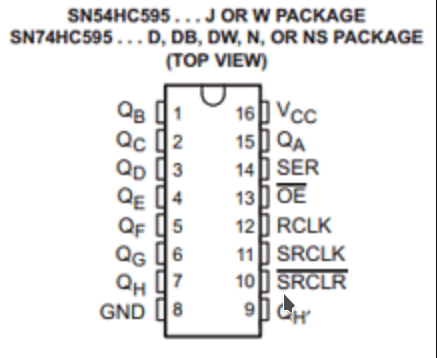
\includegraphics[width=0.8\linewidth]{images/pins}
	\figcaption{Pin-Belegung des SN54HC595N Chips}
\end{minipage}

\subsubsection{\(Q_{A} - Q_{H}\)}
Sind die jeweiligen Ausgänge, welche in dem Beispiel die LEDs mit Spannung versorgen. Wichtig dabei ist auch immer mit GND (sprich GROUND) zu verbinden:

\subsubsection{GND}
Der GROUND Anschluss des Chips. Muss immer mit dem GROUND Ports des STM-Boards verbunden sein.

\subsubsection{\(V_{CC}\)}
Muss mit dem 3Volt Anschluss vom STM-Board verbunden werden, damit der Chip genug, aber nicht zuviel Spannung bekommt.

\subsubsection{SER}
Dieser Port wird benötigt für die sogenannte ''MOSI-Verbindung'' (\textbf{M}aster \textbf{O}ut - \textbf{S}lave \textbf{I}n) . Er wird dafür verwendet Board Daten an den Chip zu senden. 
Er muss mit dem Port \verb|PA11| Pin am Board verbunden werden.

\subsubsection{OE}
Dieser Port muss ebenfalls mit dem GROUND Port des Boards angeschlossen werden, damit der Eingang an den Ausgang geleitet wird

\subsubsection{RCLK}
Der serielle Takt, normalerweise mit GROUND verbunden, kann aber offen gelassen werden, wird durch den Strich gekennzeichnet. 

\subsubsection{SRCLK}
Die serielle Clock, noramlerweise mit PC11 verbunden

\subsubsection{SRCLR}
Wie schon erwähnt, wird durch den Strich gekennzeichnet dass dieser Port offen gelassen werden kann, wird aber in dem Beispiel mit \(V_{CC}\) verbunden. 

\subsection{Konkreter Aufbau}
Zum Aufbau wurde eine externe Schaltplatte verwendet, um die Portzuweisung einfacher zu gestalten.

Bilder sind von Filip Scopulovic: 


\begin{minipage}{\linewidth}
	\centering
	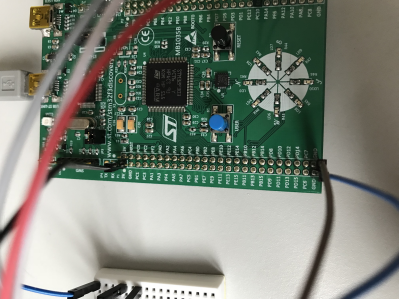
\includegraphics[width=0.8\linewidth]{images/aufbau1}
	\figcaption{Verkabelung am Board 1}
\end{minipage}

\begin{minipage}{\linewidth}
	\centering
	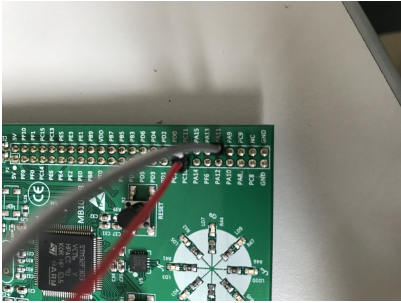
\includegraphics[width=0.8\linewidth]{images/aufbau2}
	\figcaption{Verkabelung am Board 2}
\end{minipage}

\begin{minipage}{\linewidth}
	\centering
	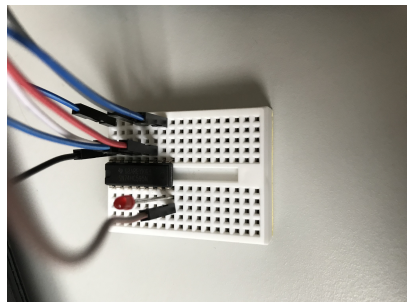
\includegraphics[width=0.8\linewidth]{images/aufbau3}
	\figcaption{Verkabelung auf der Schaltplatte inklusive der Portanschliessung des Chips}
\end{minipage}

\begin{minipage}{\linewidth}
	\centering
	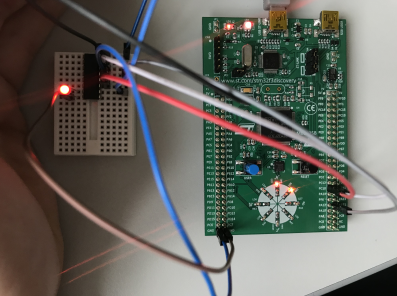
\includegraphics[width=0.8\linewidth]{images/aufbau4}
	\figcaption{Gesamter Aufbau}
\end{minipage}

\section{Umsetzung}
\subsection{GPIOC konfigurieren}
Zuerst müssen der Pins des Ports C konfiguriert werden:

\begin{lstlisting}[language=C]
void configureGPIOC () {
	__GPIOC_CLK_ENABLE();
	// Pins 10, 11 und 12 konfigurieren
	GPIO_InitStruct.Pin = GPIO_PIN_10| GPIO_PIN_11| GPIO_PIN_12;
	GPIO_InitStruct.Mode = GPIO_MODE_AF_PP;
	GPIO_InitStruct.Pull = GPIO_PULLDOWN;
	GPIO_InitStruct.Speed = GPIO_SPEED_HIGH;
	GPIO_InitStruct.Alternate = GPIO_AF6_SPI3;
	HAL_GPIO_Init(GPIOC, &GPIO_InitStruct);
}
\end{lstlisting}

\subsection{GPIOA konfigurieren}
Natürlich müssen auch die Pins des Ports A initialisiert werden:
\begin{lstlisting}[language=C]
void configureGPIOA () {
	__GPIOA_CLK_ENABLE();
	GPIO_InitStruct.Pin = GPIO_PIN_11;
	GPIO_InitStruct.Mode = GPIO_MODE_OUTPUT_PP;
	GPIO_InitStruct.Pull = GPIO_PULLUP;
	GPIO_InitStruct.Speed = GPIO_SPEED_FREQ_HIGH;
	HAL_GPIO_Init(GPIOA, &GPIO_InitStruct);
}
\end{lstlisting}

\subsection{SPI konfigurieren}
Natürlich muss auch SPI initialisiert und konfiguriert werden:

\begin{lstlisting}[language=C]
void configureSPI () {
	__SPI3_CLK_ENABLE() ;
	SpiHandle.Instance = SPI3;
	SpiHandle.Init.BaudRatePrescaler = SPI_BAUDRATEPRESCALER_256;
	SpiHandle.Init.Direction = SPI_DIRECTION_2LINES;
	SpiHandle.Init.CLKPhase = SPI_PHASE_1EDGE;
	SpiHandle.Init.CLKPolarity = SPI_POLARITY_LOW;
	SpiHandle.Init.CRCCalculation = SPI_CRCCALCULATION_DISABLED;
	SpiHandle.Init.CRCPolynomial = 7;
	SpiHandle.Init.DataSize = SPI_DATASIZE_8BIT;
	SpiHandle.Init.FirstBit = SPI_FIRSTBIT_MSB;
	SpiHandle.Init.NSS = SPI_NSS_SOFT;
	SpiHandle.Init.TIMode = SPI_TIMODE_DISABLED;
	SpiHandle.Init.NSSPMode = SPI_NSS_PULSE_DISABLED;
	SpiHandle.Init.CRCLength = SPI_CRC_LENGTH_8BIT;
	SpiHandle.Init.Mode = SPI_MODE_MASTER;
	rc = HAL_SPI_Init(&SpiHandle);
}
\end{lstlisting}

\clearpage
\subsection{main()}
Es wurden nun alle Funktionen geschrieben um alle benötigten Ports und Schnittstellen zu initialisieren. Nun muss eine main Methode geschrieben, welche 1. Alle diese Funktion aufruft und 2. den eigentlichen Code ausführt, welcher die LED zum blinken bringt:

\begin{lstlisting}[language=C]
int main(void) {
	//zusaetlich zu den anderen Funktionen wird noch HAL_Init aufgerufen um alle Treiber zu starten fuer den HAL driver
	HAL_Init();
	configureGPIOC ();
	configureGPIOA ();
	configureSPI ();
	//Es wird eine int Variable erstellt
	uint8_t data = 0;
	for(;;) {
		// Der ~ Operator inversiert alle Bits einer Variable, in dem konkreten Beispiel wird bei jedem Durchlauf der while-true loop data auf 1 gesetzt wenn es davor 0 war, und auf 0 gesetzt wenn es davor 0 war. Dadurch blinkt die LED alle 5 sekunden auf, weil bei SPI_Transmit ein Delay von 5000ms angegeben wird, zusaetzlich zu den anderen Parameter
		data = ~data ;
		HAL_StatusTypeDef rc1 = HAL_SPI_Transmit(&SpiHandle , &data , 1 , 5000) ;
	}
}
\end{lstlisting}


\subsection{Probleme}
Das Problem ist nun, wenn das Projekt ausgeführt wird, blinkt die LED nicht. Daher keine Zeit mehr übrig bleib in der Schule (zuhause besitze ich keine Kabel zum verbinden, deswegen nur die Fotos des Mitschülers), um die Konfiguration zu überprüfen, muss ich Ihnen das Protokoll leider nur so abgeben. Dadurch dass das Testen des Blinkens nicht funktioniert hat, hat es keinen Sinn gemacht sich an die Implementation der Ampel zu trauen. 